\documentclass[titlepaged,toc]{../cs-classes/cs-classes}

\title{Introduction to Robotics}
\author{Julien Carpentier\and Stéphane Caron\and Yann de Mont-Marin}

\begin{document}

\begin{abstract}
    This document is Antoine Groudiev's class notes while following the class \emph{Motion planning in robotics and graphical animation} (Planification de mouvement en robotique et en animation graphique) at the Computer Science Department of ENS Ulm. It is freely inspired by the lectures of Justin Carpentier, Stéphane Caron, and Yann de Mont-Marin.
\end{abstract}

\section{Introduction and general overview}
\subsection{What is Deep Learning?}
\subsubsection{Neural networks}
\subsubsection{Timeline of Deep Learning}
\subsubsection{Recent applications and breakthroughs}
\subsubsection{Usual setup}
\subsubsection{Required skills}
\subsubsection{Building blocks of deep learning}
\subsubsection{Why deep learning now?}

\subsection{Machine Learning pipeline}
\subsubsection{Cats vs. dogs}
\subsubsection{Typical Machine Learning setup}
\subsubsection{Training objective}

\subsection{Multi-Layer Perceptron}
\subsubsection{Definition}
\subsubsection{PyTorch implementation}
\section{Position and Orientation}
\subsection{Introduction}
Kinematics studies the \emph{movement} of an object -- in our case of a robot -- without taking into acount the \emph{forces} generating it. Instead, it only handles aspects such as position, orientation, speed and momentum of bodies in movement.

Consider for instance a robotic arm. We can design a simplified scheme of the robot and its environment, to create a kinematic pipeline and reference frames associated to each of these objects.

\begin{figure}[H]
    \centering
    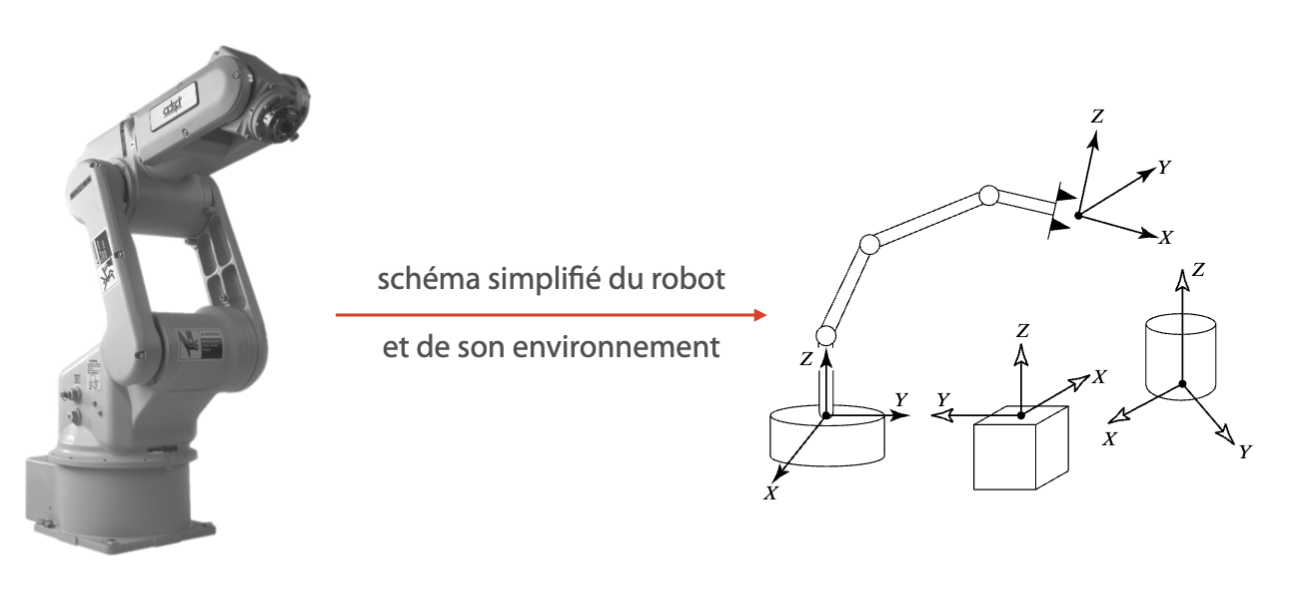
\includegraphics[width=.6\textwidth]{position/arm-scheme.png}
    \caption{Simplified scheme of the robot, the kinematic pipeline and reference frames.}
\end{figure}

\emph{Direct kinematics} allows to compute the position and orientation of the terminal organ given, for instance, the angles of the articulations.

\begin{figure}[H]
    \centering
    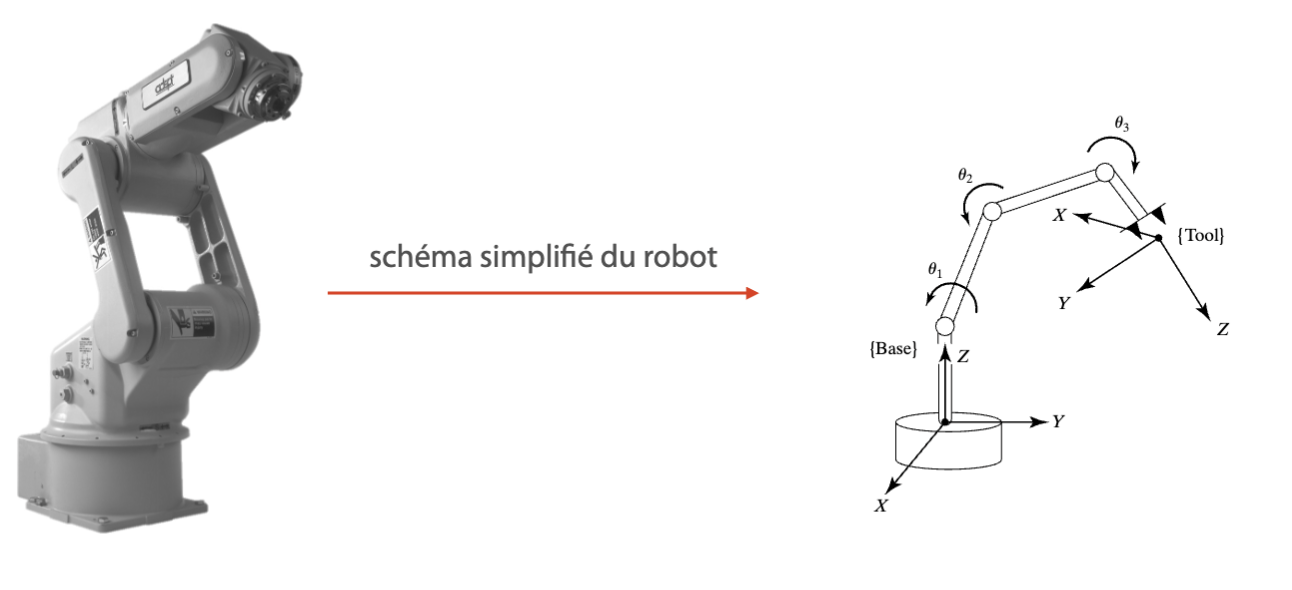
\includegraphics[width=.6\textwidth]{position/direct-kinematic.png}
\end{figure}

\emph{Invert kinematics} answers the question the other way around: given the position and orientation of a boyd, how can we compute the values of the articulations angles. Invert kinematics is used for instance for trajectory tracking: given a reference trajectory, how can we compute the speed of the articulations?

\subsection{Points, frames and transformations}
\subsubsection{Position of a point in space}
Once that a reference frame $\{A\}$ is defined, we can localize any point of the universe given a \emph{position vector}:
\begin{figure}[H]
    \centering

    \begin{minipage}{0.4\textwidth}
        \begin{equation*}
            \prescript{A}{}{P} = \begin{bmatrix}
                p_x \\ p_y \\ p_z
            \end{bmatrix}
        \end{equation*}
    \end{minipage}
    \begin{minipage}{0.4\textwidth}
        \centering
        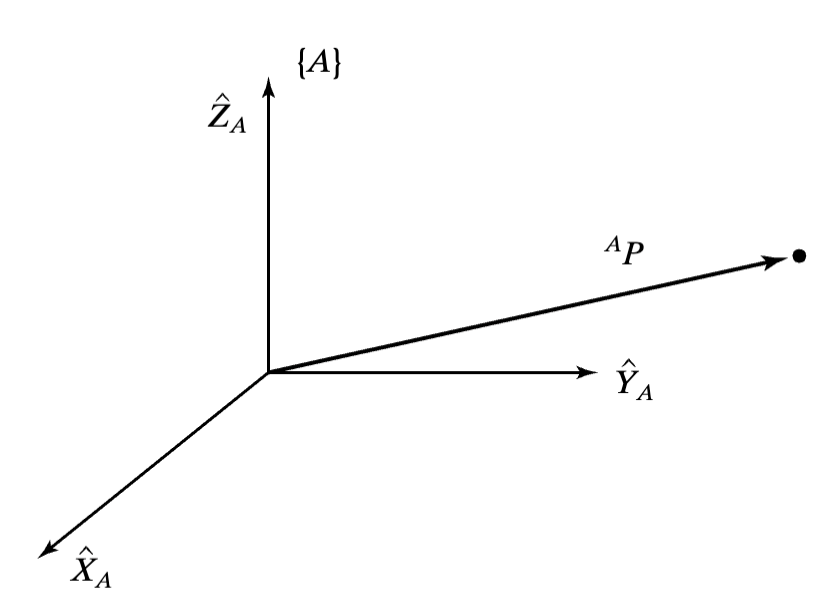
\includegraphics[width=.8\textwidth]{position/position-frame.png}
    \end{minipage}
    \caption{Vector and position of the point established in the frame $\{A\}$.}
\end{figure}

\subsubsection{Position and orientation of a body in space}
To define the orientation of a body in space, we need to define a reference frame $\{B\}$ attached to this body. The orientation is therefore defined as the expression of this coordinate system in the reference frame $\{A\}$.
\begin{figure}[H]
    \centering

    \begin{minipage}{0.5\textwidth}
        \begin{equation*}
            \prescript{A}{B}{R} = \begin{bmatrix}
                \prescript{A}{}{\hat{X}}_B & \prescript{A}{}{\hat{Y}}_B & \prescript{A}{}{\hat{Z}}_B
            \end{bmatrix}
            = \begin{bmatrix}
                r_{11} & r_{12} & r_{13} \\
                r_{21} & r_{22} & r_{23} \\
                r_{31} & r_{32} & r_{33}
            \end{bmatrix}
        \end{equation*}
    \end{minipage}
    \begin{minipage}{0.4\textwidth}
        \centering
        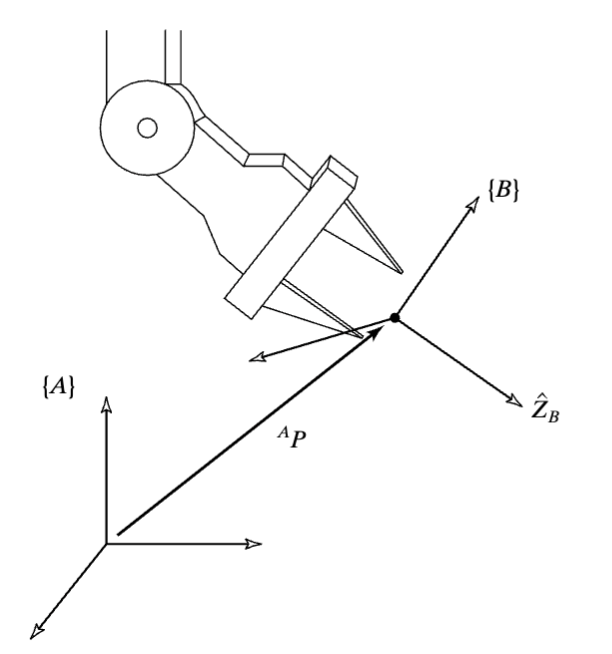
\includegraphics[width=.8\textwidth]{position/body-orientation.png}
    \end{minipage}
    \caption{Expression of the coordinate system $\{B\}$ in the reference frame $\{A\}$, and the associated position and orientation of the body.}
\end{figure}
Each element of the matrix $\prescript{A}{B}{R}$ is the scalar product between the vectors of the two coordinate systems $\{B\}$ and $\{A\}$:
\begin{equation*}
    \prescript{A}{B}{R} = \begin{bmatrix}
        \prescript{A}{}{\hat{X}}_B & \prescript{A}{}{\hat{Y}}_B & \prescript{A}{}{\hat{Z}}_B
    \end{bmatrix}
    = \begin{bmatrix}
        \hat{X}_B\cdot\hat{X}_A & \hat{Y}_B\cdot\hat{X}_A & \hat{Z}_B\cdot\hat{X}_A \\
        \hat{X}_B\cdot\hat{Y}_A & \hat{Y}_B\cdot\hat{Y}_A & \hat{Z}_B\cdot\hat{Y}_A \\
        \hat{X}_B\cdot\hat{Z}_A & \hat{Y}_B\cdot\hat{Z}_A & \hat{Z}_B\cdot\hat{Z}_A
    \end{bmatrix}
\end{equation*}
The lines correspond to the axes of the frame $\{A\}$ expressed in the frame $\{B\}$. Note that the invert of a rotation matrix is its transpose:
\begin{equation*}
    \prescript{A}{B}{R}^T = \prescript{A}{B}{R}^{-1} = \prescript{B}{A}{R}
\end{equation*}

\subsubsection{Rotation matrices}
We showed that the orientation of the body in space could be expressed as a 3-dimensional rotation matrix. The group of 3-dimensional rotation matrices is denoted $\SO(3)$, and is composed of all the matrices that are orthonormal, that is orthogonal and with a determinant equal to 1:
\begin{equation}
    \SO(3) = \set{R\in\mathcal{M}_{3}(\R)}{RR^T=I_3 \text{ and } \det(R) = +1}
\end{equation}
If we write:
\begin{equation*}
    R = \begin{bmatrix}
        \hat{X} & \hat{Y} & \hat{Z}
    \end{bmatrix}
\end{equation*}
Then $R\in\SO(3)$ if and only if:
\begin{equation*}
    \begin{cases}
        \hat{X}\cdot\hat{Y} = 0 \\
        \hat{Y}\cdot\hat{Z} = 0 \\
        \hat{Z}\cdot\hat{X} = 0 \\
    \end{cases}
    \quad\text{and}\quad
    \begin{cases}
        \hat{X}\cdot\hat{X} = 1 \\
        \hat{Y}\cdot\hat{Y} = 1 \\
        \hat{Z}\cdot\hat{Z} = 1 \\
    \end{cases}
\end{equation*}
Note that we have 9 degrees of freedom and 6 independent constraints, so the group $\SO(3)$ is 3-dimensional.

\subsection{Rotation representations}
There are several ways to represent a rotation matrix, each with its own advantages and drawbacks. The most common representations are:
\begin{itemize}
    \item Orthonormal 3 by 3 matrices --- 9 components
    \item Euler angles --- 3 components
    \item Axis-angle representation --- 3 components
    \item Quaternions --- 4 components
\end{itemize}
The number of components used to be an important factor when computers were slow and memory was expensive. Nowadays, the choice of representation is more about the ease of use and the properties of the representation.

\subsubsection{Euler angles}
Each rotation can be represented by the composition of three elementary rotations around the fixed axes of the frame $\{A\}$.
\begin{figure}[H]
    \centering
    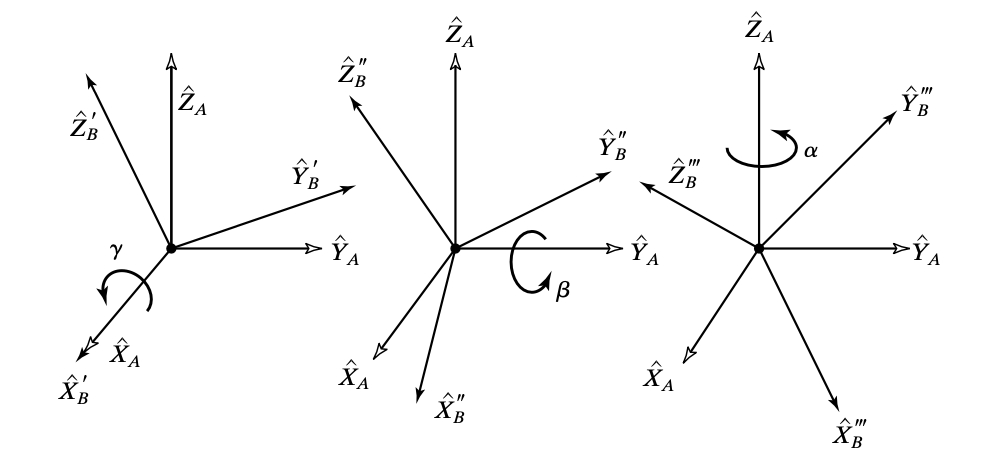
\includegraphics[width=.6\textwidth]{position/euler-angles.png}
    \caption{Euler angles representation of a rotation.}
\end{figure}
In terms of rotation matrices, any rotation matrix can be written as $\prescript{A}{B}{R}(\gamma, \beta, \alpha)$, defined by:
\begin{align*}
    \prescript{A}{B}{R}(\gamma, \beta, \alpha) &= R_Z(\alpha)R_Y(\beta)R_X(\gamma)\\
    &= \begin{bmatrix}
        \cos\alpha & -\sin\alpha & 0 \\
        \sin\alpha & \cos\alpha & 0 \\
        0 & 0 & 1
    \end{bmatrix}
    \begin{bmatrix}
        \cos\beta & 0 & \sin\beta \\
        0 & 1 & 0 \\
        -\sin\beta & 0 & \cos\beta
    \end{bmatrix}
    \begin{bmatrix}
        1 & 0 & 0 \\
        0 & \cos\gamma & -\sin\gamma \\
        0 & \sin\gamma & \cos\gamma
    \end{bmatrix}
\end{align*}
The Euler angles are not unique, as the same rotation can be represented by different sets of Euler angles. This is called gimbal lock, and is a major drawback of the Euler angles representation.

We can also express the Euler angles given the rotation matrix:
\begin{align*}
    \prescript{A}{B}{R}(\gamma, \beta, \alpha) = \begin{bmatrix}
        r_{11} & r_{12} & r_{13} \\
        r_{21} & r_{22} & r_{23} \\
        r_{31} & r_{32} & r_{33}
    \end{bmatrix}
    \implies
    \begin{cases}
        \beta = \atantwo(-r_{31}, \sqrt{r_{11}^2+r_{21}^2}) \\
        \alpha = \atantwo(r_{21}/\cos\beta, r_{11}/\cos\beta) \\
        \gamma = \atantwo(r_{32}/\cos\beta, r_{33}/\cos\beta)
    \end{cases}
\end{align*}

\subsubsection{Axis-angle and quaternions}
We are given a vector $\vec{k}$ and an angle $\theta$; the rotation represented by these two elements is the rotation of angle $\theta$ around the axis $\vec{k}$. We can define:
\begin{equation*}
    \begin{cases}
        \epsilon_1 = k_x\sin\frac{\theta}{2} \\
        \epsilon_2 = k_y\sin\frac{\theta}{2} \\
        \epsilon_3 = k_z\sin\frac{\theta}{2} \\
        \epsilon_4 = \cos\frac{\theta}{2}
    \end{cases}
\end{equation*}
we have $\epsilon_1^2+\epsilon_2^2+\epsilon_3^2+\epsilon_4^2=1$, creating a unit quaternion. The rotation matrix associated to the quaternion is:
\begin{equation*}
    R_\epsilon = \begin{bmatrix}
        1-2\epsilon_2^2-2\epsilon_3^2 & 2(\epsilon_1\epsilon_2-\epsilon_3\epsilon_4) & 2(\epsilon_1\epsilon_3+\epsilon_2\epsilon_4) \\
        2(\epsilon_1\epsilon_2+\epsilon_3\epsilon_4) & 1-2\epsilon_1^2-2\epsilon_3^2 & 2(\epsilon_2\epsilon_3-\epsilon_1\epsilon_4) \\
        2(\epsilon_1\epsilon_3-\epsilon_2\epsilon_4) & 2(\epsilon_2\epsilon_3+\epsilon_1\epsilon_4) & 1-2\epsilon_1^2-2\epsilon_2^2
    \end{bmatrix}
\end{equation*}

The invert operation is also simple to compute:
\begin{align*}
    \prescript{A}{B}{R}(\gamma, \beta, \alpha) = \begin{bmatrix}
        r_{11} & r_{12} & r_{13} \\
        r_{21} & r_{22} & r_{23} \\
        r_{31} & r_{32} & r_{33}
    \end{bmatrix}
    \implies
    \begin{cases}
        \epsilon_1 = \frac{r_{32}-r_{23}}{4\epsilon_4} \\
        \epsilon_2 = \frac{r_{13}-r_{31}}{4\epsilon_4} \\
        \epsilon_3 = \frac{r_{21}-r_{12}}{4\epsilon_4} \\
        \epsilon_4 = \frac{1}{2}\sqrt{1+r_{11}+r_{22}+r_{33}}
    \end{cases}
\end{align*}

\subsection{Angular velocity}
The angular velocity of a body is a vector that describes the rotation of the body in space. It is defined as the derivative of the rotation matrix with respect to time. Angular velocity matrices are skew-symmetric matrices, i.e. matrices of the tangent space of $\SO(3)$, denoted $\so(3)$:
\begin{equation*}
    \so(3) = \set{W\in\mathcal{M}_3(\R)}{W^\tp=-W} = \set{\begin{bmatrix}
        0 & -w_z & w_y \\
        w_z & 0 & -w_x \\
        -w_y & w_x & 0
    \end{bmatrix}}{w_x, w_y, w_z\in\R}
\end{equation*}
Indeed, consider the rotation matrix $R(t)\in\SO(3)$, and denote $\dot R(t) = \partfrac{R(t)}{t}$ the derivative of $R(t)$ with respect to time. We have:
\begin{align*}
    R(t)R(t)^\tp &= I_3 \\
    \dot RR^\tp + R\dot R^\tp &= 0_3 \\
    \dot RR^\tp &= -R\dot R^\tp \\
    \dot RR^\tp &= -\left(\dot RR^\tp\right)^\tp \\
\end{align*}
Hence, by defining $W := \dot RR^\tp$, we have $W\in\so(3)$.

Note that $R(t)$ is the solution of the differential equation $\dot R = WR$, with $R(0)=R_0\in\SO(3)$. The solution is:
\begin{equation*}
    R(t) = R_0\exp(Wt) \quad\text{where}\quad \exp(Wt) = \sum_{n=0}^{+\infty}\frac{(Wt)^n}{n!}
\end{equation*}
This gives us a new parameterization of the group $\SO(3)$, using the angular velocity matrices. Recall that a matrix $W\in\so(3)$ is associated to a vector $w=(w_x, w_y, w_z)\in\R^3$; we denote $\hat{w}=W$. The main question associated to this representation is to compute the infinite sum of the exponential function:
\begin{equation}
    \exp(tW)=\sum_{n=0}^{+\infty}\frac{(tW)^n}{n!}
\end{equation}
We can use the fact that any skew-symmetric matrix $W\in\so(3)$ is nilpotent, i.e. there exists an integer $n\in\N$ such that $W^n=0_3$. This allows us to compute the exponential function:
\begin{equation*}
    \hat{w}=W=\begin{bmatrix}
        0 & -w_z & w_y \\
        w_z & 0 & -w_x \\
        -w_y & w_x & 0
    \end{bmatrix} = w \times \cdot
\end{equation*}
Therefore, $\hat{w}^2=ww^\tp-I_3$, and $\hat{w}^3=-\hat{w}$. We can then regroup the different terms of the exponential function, by transforming the exponents greater than 3:
% TODO: detail computation
\begin{equation}
    \exp(tW)=I_3+\sin(t)\hat{w}+\frac{1-\cos(t)}{t}\hat{w}^2
\end{equation}

\subsection{Exponential and logarithm map}
We saw that the exponential map is an application from the tangent space of $\SO(3)$, $\so(3)$ to the group $\SO(3)$, defined by:
\begin{align*}
    \exp:\so(3)&\longrightarrow\SO(3)\\
    tW&\longmapsto\exp(tW) = I_3 + \sin(t)\hat{w} + \frac{1-\cos(t)}{t}\hat{w}^2
\end{align*}
This function is surjective and $2\pi$-periodic.

We can define a reciprocal function, the logarithm map, that is the inverse of the exponential map:
\begin{equation*}
    \log:R\in\SO(3)\longrightarrow w\in\so(3)
\end{equation*}
Note that
\begin{equation*}
    \norm{w}=\cos^{-1}\left(\frac{\Tr(R)-1}{2}\right)
\end{equation*}
and therefore:
\begin{equation*}
    w=\frac{\norm{w}}{2\sin(\norm{w})}\begin{bmatrix}
        r_{32}-r_{23} \\
        r_{13}-r_{31} \\
        r_{21}-r_{12}
    \end{bmatrix}
\end{equation*}

This gives us a way to compute the distance between two rotations:
\begin{equation*}
    d(R_1, R_2) = \norm{\log(R_1^\tp R_2)}
\end{equation*}
Such a construction comes handy when we want to minimize the distance between two rotations, for instance in the context of trajectory tracking.

\subsection{Rigid Body Transformations}

\section{Forward Kinematics}
\emph{Forward kinematics} allows to compute the position and orientation of the kinematic chain given the joint parameters (e.g. angles, lengths, etc.). For instance, we can compute the position and orientation of the terminal organ given the angles of the articulations.
\begin{figure}[H]
    \centering
    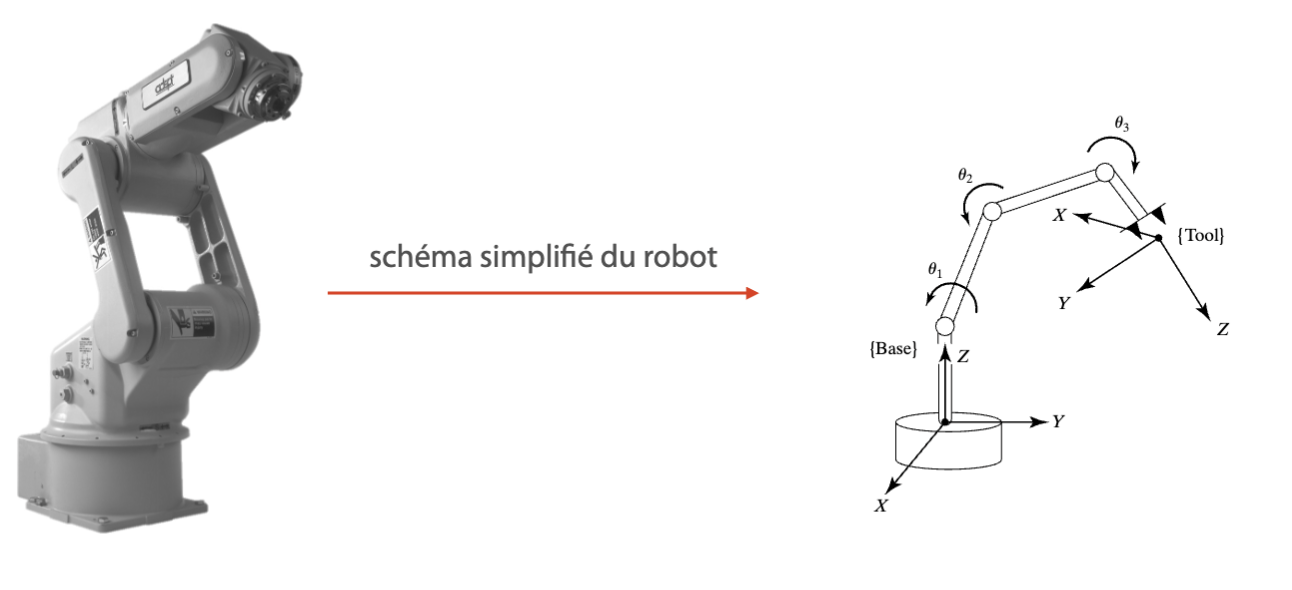
\includegraphics[width=.7\textwidth]{position/direct-kinematic.png}
\end{figure}

The kinematic chain is composed of rigid bodies interconnect by joints. The joins define the degrees of freedom of the cinematic chain, which are the parameters that we can control.
\begin{figure}[H]
    \centering
    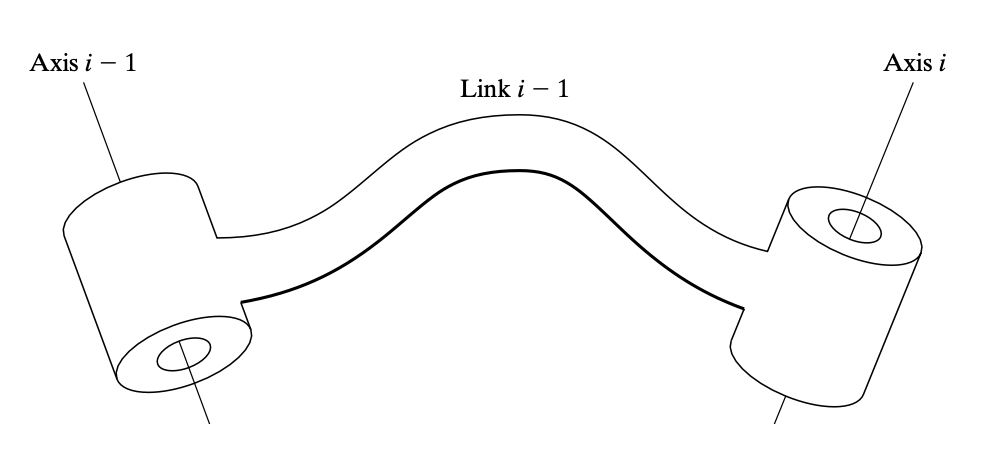
\includegraphics[width=.5\textwidth]{forward-kinematics/kinematic-chain.png}
\end{figure}

\subsection{Articulations and joint speed}
\subsubsection{Joint types and degrees of freedom}
The topology of the articulation between two rigid bodies defines the degrees of freedom of the joint.
\begin{figure}[H]
    \centering
    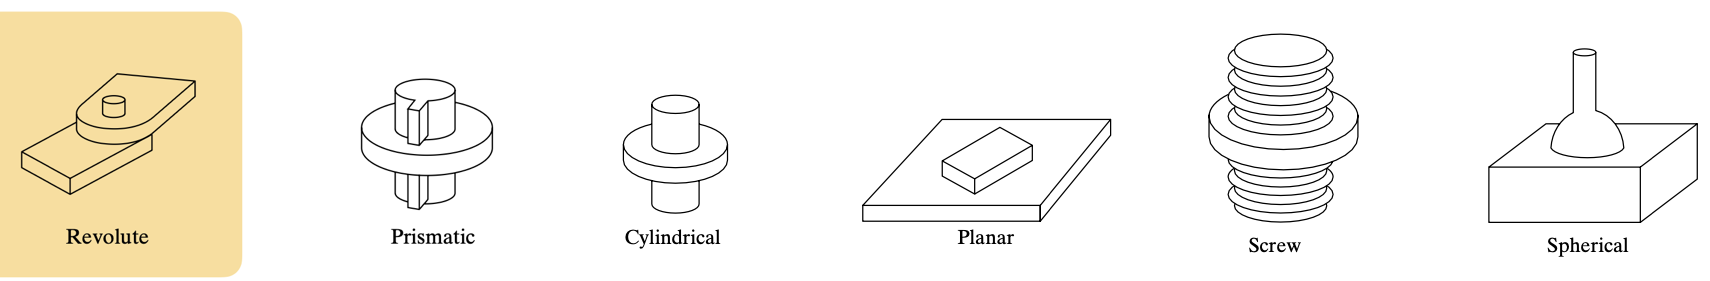
\includegraphics[width=.9\textwidth]{forward-kinematics/joints.png}
    \caption{Example of possible joints.}
\end{figure}
Each joint can be represented as a function $K_i$ from a configuration space $Q_i$ to the Special Euclidean Group $\SE(3)$:
\begin{equation*}
    \begin{aligned}
        K_i: Q_i &\longrightarrow \SE(3)\\
        q &\longmapsto M_i(q_i)
    \end{aligned}
\end{equation*}

Consider for instance the revolute joint, which constrains the motion of two bodies around a fixed axis. It is parameterized by the angle $\theta\in\R$, therefore the configuration space is $Q_i=\Sb^1\simeq\R$ (one degree of freedom). The function $K_i$ is then defined as:
\begin{equation*}
    \begin{aligned}
        K_i: \Sb^1\simeq\R &\longrightarrow \SE(3)\\
        q &\longmapsto \begin{bmatrix}
            \cos  & -\sin q & 0 & 0\\
            \sin q & \phantom{-}\cos q & 0 & 0\\
            0 & 0 & 1 & 0\\
            0 & 0 & 0 & 1
        \end{bmatrix}
    \end{aligned}
\end{equation*}

\subsubsection{Joint speed}
The change of configuration of the joint comes from the joint speed, which is the derivative of the joint parameter with respect to time. Consider the relative position of the articulation between the two adjactent frames, given by:
\begin{equation*}
    \begin{aligned}
        K_i : Q_i &\longrightarrow \SE(3)\\
        q_i &\longmapsto M_i(q_i)
    \end{aligned}
\end{equation*}
The relative speed of the joint generated by the articulation is given by:
\begin{equation*}
    \begin{aligned}
        k_i:T_{q_i}Q_i &\longrightarrow \se(3)\\
        (q_i, \dot{q}_i) &\longmapsto v_i(q_i) = S_i(q_i)\dot{q}_i
    \end{aligned}
\end{equation*}
for some transformation $S_i$.

In the case of the revolute joint, the speed of the joint is given by:
\begin{equation*}
    \begin{aligned}
        k_i: T_q\Sb^1\simeq\R^2 &\longrightarrow \se(3)\\
        (q, \dot{q}) &\longmapsto (v, w) = \left(
            \begin{bmatrix}
                0\\0\\0
            \end{bmatrix}, \begin{bmatrix}
                0\\0\\\dot{q}
            \end{bmatrix}\right)
    \end{aligned}
\end{equation*}
Hence, we have:
\begin{equation*}
    S_i(q) = \begin{bmatrix}
        0\\0\\0\\0\\0\\1
    \end{bmatrix} \in \mathscr{M}_{6, 1}(\R)
\end{equation*}
which gives us $S_i(q)\dot{q}=(v,w)$ as expected.

\subsection{Direct geometry}
We aim to compute the position and orientation of the terminal organ given the joint parameters. We can do so by computing the transformation matrix of each body in the kinematic chain, and then multiplying them to get the transformation matrix of the terminal organ.

\subsubsection{Transformation matrix}
Given an articulation $i$, we can compute the relative position of the associated frame $i$ with respect to the frame $i-1$ using the function $K_i$:
\begin{equation*}
    \prescript{i-1}{}{M_i(q_i)} = \prescript{i-1}{}{P_iK_i(q_i)}
\end{equation*}
We can combine the transformations of all the bodies in the kinematic chain to get the transformation matrix of the terminal organ:
\begin{equation*}
    \begin{aligned}
        \prescript{0}{}{K_n} : \bigtimes_{i=1}^n Q_i &\longrightarrow \SE(3)\\
        q=(q_1, \dots, q_n) &\longmapsto \bigtimes_{i=1}^n \prescript{i-1}{}{M_i(q_i)}
    \end{aligned}
\end{equation*}
Therefore, the configuration space can be read as the product of the configuration spaces of each joint:
\begin{equation*}
    Q = \bigtimes_{i=1}^N Q_i \simeq \R^{\sum_{i=1}^N n_i}
\end{equation*}
where $N$ is the number of joints.

\subsubsection{Kinematic Jacobian}
Our goal is now to link the joint speed to the spatial speed of the bodies in movement. For each articulation, we have a linear mapping of the form:
\begin{equation*}
    v_i(q_i) = S_i(q_i)\dot{q_i}
\end{equation*}
This corresponds to the temporal derivative of the articular geometry:
\begin{equation*}
    \dot{M}_i(q_i)M_i^{-1}(q_i) = S_i(q_i)\dot{q}_i
\end{equation*}
Therefore, one can link the spatial speed of a body to the joint speed using the relation:
\begin{equation*}
    \prescript{0}{}{k_n}(q, \dot{q}) = \sum_{i=1}^n k_i(q_i, \dot{q}_i) = \underbrace{\begin{bmatrix}
        S_1(q_1) \cdots S_n(q_n)
    \end{bmatrix}}_{J(q)}
    \begin{bmatrix}
        \dot{q}_1\\\vdots\\\dot{q}_n
    \end{bmatrix}
\end{equation*}
\section{Inverse Kinematics}
\emph{Inverse Kinematics} aims at finding joint parameters that achieve a desired end-effector pose. This is a more complex problem than forward kinematics, as it is not always possible to find a solution, and when it is, there may be multiple solutions.
\begin{figure}[H]
    \centering
    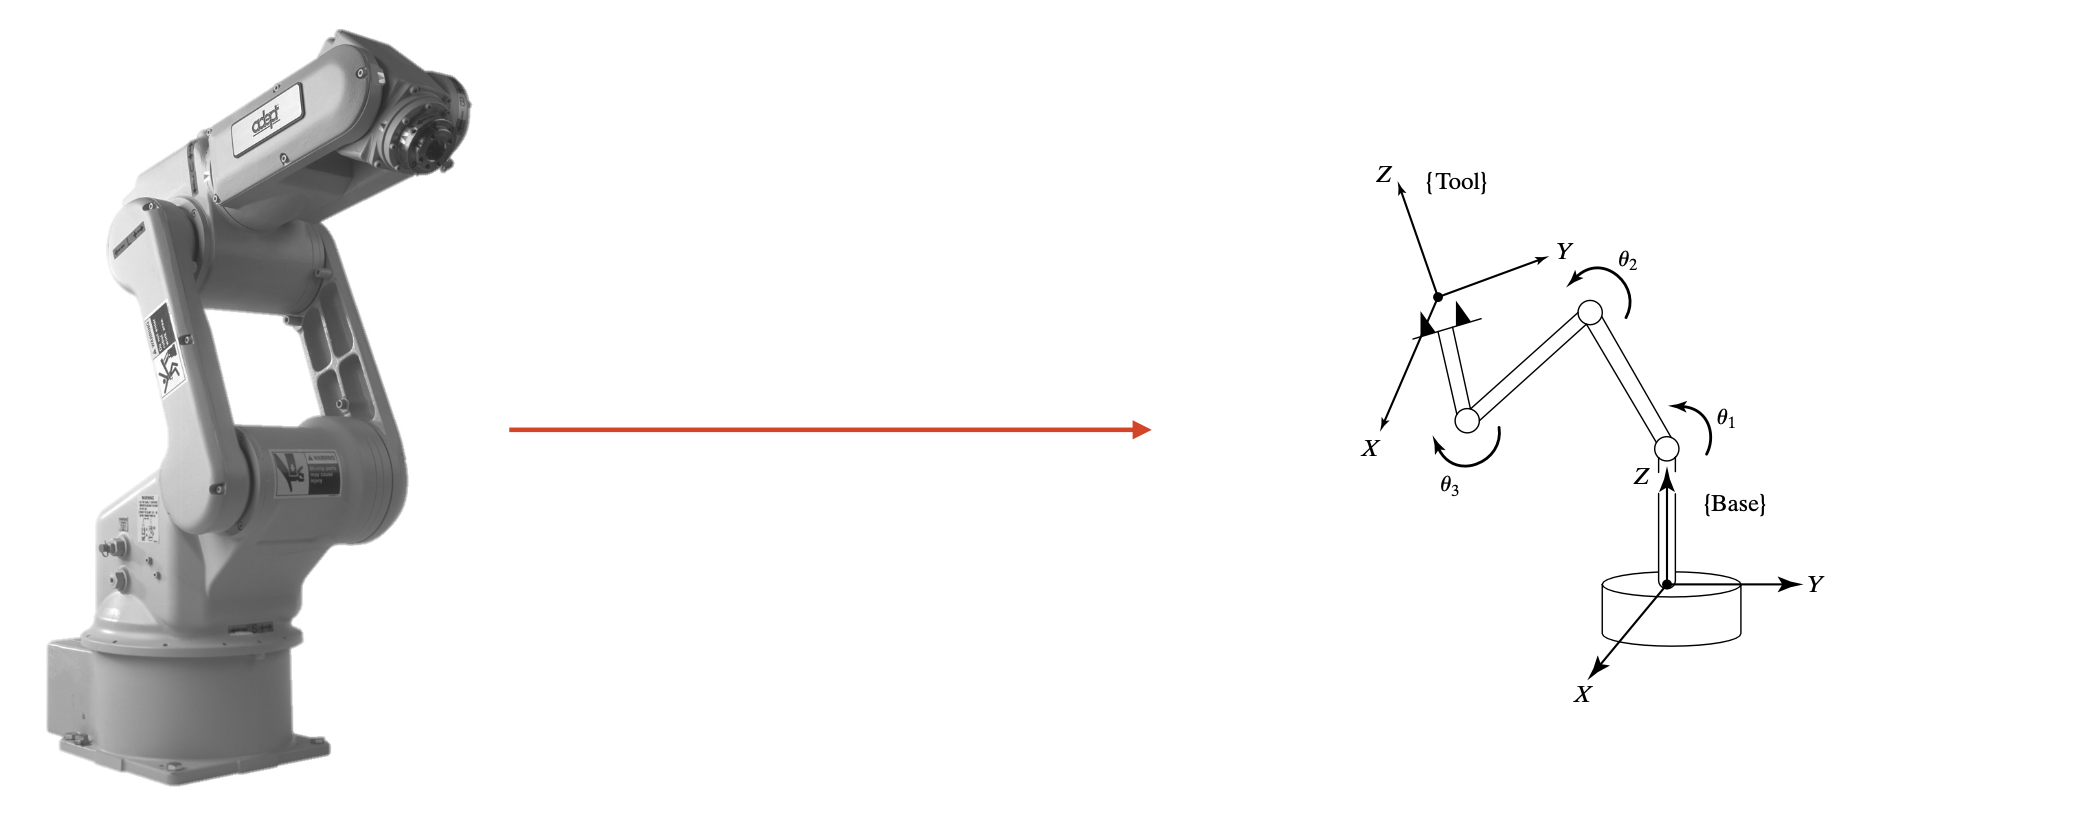
\includegraphics[width=0.8\textwidth]{inverse-kinematics/inverse-kinematics.png}
\end{figure}

\subsection{Optimization problem and resolution}
Given a target position $M^*$ for the end-effector, we aim at solving the following distance minimization problem:
\begin{equation*}
    \min_{q\in Q} d(\prescript{0}{}{K_n(q)}, M^*)
\end{equation*}
Using the logarithm distance, we can rewrite the problem as:
\begin{equation}
    \min_{q\in Q} \norm{\log(\prescript{0}{}{K_n(q)}^{-1}M^*)}
\end{equation}
We can cast this initial problem $\min_{q\in Q} \norm{\log(\prescript{0}{}{K_n(q)}^{-1}M^*)}$ as a more general optimization problem:
\begin{equation*}
    \min_{x\in\R^n}\frac{1}{2}\norm{f(x)}_2^2
\end{equation*}
We aim at iteratively solving this optimization problem. A first-order linear approximation of $f$ around $x$ is given by:
\begin{equation*}
    f(x+p)=f(x)+\underbrace{\partfrac{f}{x}(x)}_{J(x)}p
\end{equation*}
Hence:
\begin{equation*}
    \min_{p\in\R^n}\frac{1}{2}\norm{f(x_0+p)}_2^2 = \min_{p\in\R^n}\frac{1}{2}\norm{f(x)+J(x)p}_2^2
\end{equation*}
We can now solve the optimization problem by setting the gradient of the objective function to zero:
\begin{equation*}
    \begin{aligned}
        &\nabla_p\left(\frac{1}{2}\norm{f(x)+J(x)p^*}_2^2\right)=0\\
        \iff &J(x)^\tp (f(x)+J(x)p^*) = 0\\
        \iff &p^* = -(J(x)^\tp J(x))^{-1}J(x) f(x)\\
        \iff &p^* = -J(x)^+ f(x)
    \end{aligned}
\end{equation*}
where $J(x)^+$ is the \emph{Moore-Penrose pseudoinverse} of $J(x)$. We can then iteratively update:
\begin{equation*}
    x_{k+1} = x_k + \alpha p_k
\end{equation*}
until we obtain $\norm{J(x)^\tp f(x)}\leq\epsilon^*$, where $\epsilon^*>0$ is a fixed precision we aim at achieving. This iterative method is known as the \emph{Newton-Raphson} method. If we work on a differential manifold, we can use instead:
\begin{equation*}
    q_{k+1}=q_l\oplus\alpha p_k
\end{equation*}

\subsection{Trajectory tracking}
We can extend the previous method to track a trajectory $M(t)$: we want to compute the joint speeds $\dot{q}$ that track the trajectory as closely as possible. Consider a continuous and differentiable time trajectory $M^*$:
\begin{equation*}
    \begin{aligned}
        M^*:[0, T]&\longrightarrow \SE(3)\\
        t&\longmapsto M^*(t)
    \end{aligned}
\end{equation*}
We are also given the corresponding spatial (linear and angular) velocity of the end-effector $v^*$:
\begin{equation*}
    \begin{aligned}
        v^*:[0, T]&\longrightarrow\se(3)\\
        t&\longmapsto v^*(t)
    \end{aligned}
\end{equation*}

At each instant $t$, the forward kinematics of the robot give us the current end-effector pose $M(t)$ and the corresponding Jacobian $J(t)$:
\begin{equation*}
    M(q(t)) = \bigtimes_{i=0}^n K_i(q_i(t)) \in\SE(3)
    \quad\text{and}\quad
    v(t) = J(q(t))\dot{q}(t)\in\se(3)
\end{equation*}
Using the angular speed of the joints $\dot{q}(t)$, we can control the position $q(t)$ of the joints. Our goal is to minimize the gap between the position and speed of the end-effector $(M(q(t)), v(q(t), \dot{q}(t)))$ and the desired trajectory $(M^*(t), v^*(t))$.

The error can be computed using the following cost function:
\begin{equation*}
    e(t, q(t)) = M(q(t)) \ominus M^*(t) = \log_{\SE(3)}\left(M^*(t)^{-1}M(q(t))\right)
\end{equation*}
The error in velocity space is given by:
\begin{equation*}
    \dot{e}(t, q(t), \dot{q}(t)) = v(q(t), \dot{q}(t)) - v^*(t) = J(q(t))\dot{q}(t) - v^*(t)
\end{equation*}
We define the error correction profile as:
\begin{equation*}
    \dot{e}(t, q(t), \dot{q}(t)) = -\lambda e(t, q(t))
\end{equation*}
for some $\lambda>0$. This finally gives us the following optimization problem:
\begin{equation}
    \boxed{\min_{\dot{q}(t)} \frac{1}{2}\norm{\dot{e}+\lambda e}_2^2}
\end{equation}
\section{Direct and Inverse Dynamics}
Previously, we studied \emph{kinematics}, which describes the motion of a robot without considering the forces that cause it. We now turn to \emph{dynamics}, which studies the \emph{forces} that cause the motion. 

Similarly to kinematics, dynamics can be divided into two problems: the \emph{direct dynamics} problem and the \emph{inverse dynamics} problem. The \emph{direct dynamics} problem consists in finding the motion of a robot given the forces applied to it. Conversely, the goal of \emph{inverse dynamics} is to minimize the gap between the position and speed of the end-effector and the desired trajectory, while taking into account the dynamics of the robot.

\subsection{Physical equations}
The motion of a robot is governed by the laws of physics. The \emph{Newton-Euler} equations describe the motion of a rigid body in space. They are a set of differential equations that relate the forces and torques applied to the body to its translational and rotational motion. The equations are given by:
\begin{equation}
    \tag{Newton's equation}
    m_k\underline{\ddot{x}}_k = f_k
\end{equation}
for the translational motion, and:
\begin{equation}
    \tag{Euler's equation}
    I_k\underline{\dot{\omega}}_k + \underline{\omega}_k\times I_k\underline{\omega}_k = \tau_k
\end{equation}
for the rotational motion. Here, $m_k$ is the mass of the body, $f_k$ is the force applied to it, $I_k$ is the inertia matrix, $\underline{\omega}_k$ is the angular velocity, and $\tau_k$ is the torque applied to the body. The equations are written in the body frame of the body $k$, whose origin coincides with the body's center of mass.

Almost all physical problems, from mechanics to relativity, follow the \emph{least-action principle}. This principle states that the actual motion of a system is the one that minimizes a certain quantity, called the \emph{action}. In mechanics, it corresponds to the minimization of the integral of the kinetic-potential energies over time.

We can define $\Ds$ to be a kinetic metric of least deviation between the actual motion of the robot and the desired motion:
\begin{equation}
    \Ds := \sum_{k=1}^n \frac{1}{2}(\ddot{x}_k - \underline{\ddot{x}}_k)^\tp m_k (\ddot{x}_k - \underline{\ddot{x}}_k) + \frac{1}{2}(\dot{\omega}_k - \underline{\dot{\omega}}_k)^\tp I_k (\dot{\omega}_k - \underline{\dot{\omega}}_k)
\end{equation}
Formally, the least-action principle states that the actual motion of the robot is the one that minimizes $\Ds$. We can find the actual motion by solving the following optimization problem:
\begin{equation}
    \min_{\ddot{x}_k, \dot{\omega}_k} \Ds
\end{equation}

In the joint space, we can write the equations of motion as:
\begin{equation}
    M(q)\ddot{q} + C(q, \dot{q}) - F(q) = 0
\end{equation}
where $M(q)$ is the mass matrix, $C(q, \dot{q})$ is the Coriolis matrix, and $F(q)$ is the vector of forces applied to the joints.

\subsection{Contact forces}
The poly-articulated system dynamics is driven by the Lagrangian dynamics. If we consider the contact forces, we can write the equations of motion as:
\begin{equation*}
    \underbrace{M(q)}_{\text{Mass matrix}}\ddot{q} + \underbrace{C(q, \dot{q})}_{\text{Coriolis}} + \underbrace{G(q)}_{\text{Gravity}} = \underbrace{\tau}_{\text{Motor torque}} + \underbrace{J_c^\tp(q)\lambda_c}_{\text{External forces}}
\end{equation*}

With this equation in mind, the direct dynamics problem consists in finding the motion of the robot given the forces applied to it. Schematically, the problem can be written as:
\begin{equation*}
    \ddot{q} = \text{ForwardDynamics}(q, \dot{q}, \tau, \lambda_c)
\end{equation*}
This is used in simulation, and can be solved using the articulated body algorithm.

Conversely, the \emph{inverse dynamics} problem consists in finding the forces applied to the robot given its motion. Schematically, the problem can be written as:
\begin{equation*}
    \tau = \text{InverseDynamics}(q, \dot{q}, \ddot{q}, \lambda_c)
\end{equation*}
This is used in control, and can also be solved by integrating the equations of motion over time (recursive Newton-Euler algorithm).

Note that naive algorithms for solving the direct dynamics problem have a complexity of $O(n^3)$, which is prohibitive for large systems. However, the articulated body algorithm has a complexity of $O(n)$, which makes it tractable for large systems. Such improvements come from the structure of the mass matrix, which is often sparse since parts of the robots are not connected. Similarly, the Jacobian of the contact forces is often sparse, which can also be exploited to reduce the complexity of the problem.

An important aspect of the direct dynamics problem is the computation of $\lambda_c$. Multiple approaches, corresponding to different contact models, can be used:
\begin{itemize}
    \item Soft contact: using a spring-damper model
    \item Rigid contact: using a bilateral or unilateral contact model
    \item Mixed contact: using a relaxed contact model
\end{itemize}
we will study these models in more detail in the next sections.

\subsection{Soft contact}
The soft contact model is used when the contact between the robot and the environment is soft, i.e. when the robot can penetrate the environment. This is one of the simplest contact model, which is both very intuitive and straightforward to implement. 

The model is based on a spring-damper system, where the contact force is proportional to the penetration depth and the relative velocity between the robot and the environment. The spring will push the robot away from the environment (proportionally to the penetration $p$), while the damper will slow down the relative motion between the robot and the environment (proportionally to the speed $\dot{p}$).

We consider the parameter $k$ to be the stiffness of the spring, and $b$ to be the damping coefficient of the damper. The contact force is then given by:
\begin{equation}
    \lambda_c = \max(-k\cdot p - b\cdot\dot{p}, 0)
\end{equation}
The $\max$ function is used to ensure that the contact force is always positive, i.e. that the robot is always pushed away from the environment.

Lower values of $k$ correspond to softer contacts, while higher values of $k$ correspond to harder objects. Higher values of $d$ also mean higher energy dissipation; in the case of a trampoline, for instance, we would have a very low $d$ to allow the robot to bounce back.

Despite being simple and easy, the soft contact model is not relevant for rigid interfaces (when $k\to+\infty$). Furthermore, it requires a very stable integrator, since the equation is stiff (because of the $\max$ function).

\subsection{Rigid bilateral contacts}
\subsubsection{Optimization problem}
The rigid contact model is used when the contact between the robot and the environment is rigid, i.e. when the robot cannot penetrate the environment. It uses the least-action principle to write and solve an optimization problem: given $q$ and $\dot{q}$, we aim at retrieving $\ddot{q}$ and $\lambda_c$.

When the contact is symmetric, i.e. when the robot can push the environment and the environment can push the robot, we used the bilateral contact model. To do so, we solve the following optimization problem:
\begin{equation}
    \label{eq:bilateral-contact}
    \min_{\ddot{q}} \frac{1}{2}\norm{\ddot{q}-\ddot{q}_f}^2_{M(q)} \quad\text{s.t.}\quad c(q)=0
\end{equation}
where $c(q)$ is the contact function, $J_c(q)$ its Jacobian. The constraint $c(q)=0$ ensures that the robot is in contact with the floor. Here, we are minimizing the distance between the actual acceleration and the \emph{free acceleration} with respect to the unconstrained acceleration. This distance is measured by the metric induced by the kinetic energy (hence by the mass matrix $M(q)$). The free acceleration is the acceleration that the robot would have if it was not in contact with the floor. It can be expressed as:
\begin{equation*}
    \ddot{q}_f = M(q)^{-1}(\tau - C(q, \dot{q}) - G(q))
\end{equation*}

Note that from the constraint $c(q)=0$ we can derive by differentiation the following equation:
\begin{equation*}
    c(q)=0\implies J_c(q)\dot{q}=0 \implies J_c(q)\ddot{q} + \underbrace{\dot{J}_c(q,\dot{q})\dot{q}}_{\gamma_c(q, \dot{q})} = 0
\end{equation*}
Therefore, we can rewrite \autoref{eq:bilateral-contact} as:
\begin{equation}
    \min_{\ddot{q}} \frac{1}{2}\norm{\ddot{q}-\ddot{q}_f}^2_{M(q)} \quad\text{s.t.}\quad J_c(q)\ddot{q} + \gamma_c(q, \dot{q}) = 0
\end{equation}

\subsubsection{Solution using the KKT conditions}
The solution of this problem can be retrieved by deriving the KKT conditions\footnote{The \emph{Karush-Kuhn-Tucker (KKT) conditions} are conditions for a solution of an optimization problem to be optimal.} of the QP problem, via the so-called \emph{Lagrangian}:
\begin{equation*}
    \L(\ddot{q}, \lambda_c) = 
    \underbrace{
        \frac{1}{2}\norm{\ddot{q}-\ddot{q}_f}^2_{M(q)}
     }_{\text{cost function}} + 
     \lambda_c^\tp
     \underbrace{
        \left(J_c(q)\ddot{q} + \gamma_c(q, \dot{q})\right)
     }_{\text{equality constraint}}
\end{equation*}
where $\lambda_c$, the dual variable (or Lagrange multiplier), corresponds to the contact forces. The KKT conditions of the QP problem are given by:
\begin{align}
    \nabla_{\ddot{q}}\L &= M(q)(\ddot{q}-\ddot{q}_f) - J_c^\tp(q)\lambda_c = 0 \\
    \nabla_{\lambda_c}\L &= J_c(q)\ddot{q} + \gamma_c(q, \dot{q}) = 0
\end{align}
where the first equation represents the joint space force propagation, and the second equation translates the contact acceleration constraint.

By rearranging the equations, we obtain:
\begin{align*}
    M(q)\ddot{q} - J_c^\tp(q)\lambda_c &= \phantom{-}M(q)\ddot{q}_f\\
    J_c(q)\ddot{q} + \qquad\quad0 &= -\gamma_c(q, \dot{q})
\end{align*}
leading to the \emph{KKT dynamics equation}:
\begin{equation}
    \underbrace{\begin{bmatrix}
        M(q) & J_c^\tp(q) \\
        J_c(q) & 0
    \end{bmatrix}}_{K(q)}
    \begin{bmatrix}
        \ddot{q} \\
        -\lambda_c
    \end{bmatrix} =
    \begin{bmatrix}
        M(q)\ddot{q}_f \\
        -\gamma_c(q, \dot{q})
    \end{bmatrix}
\end{equation}
Note that there might be one, multiple, or no solution to this problem. This depends on whether $J_c(q)$ is full rank, not full rank, or if $\gamma_c(q, \dot{q})$ is not in the range space of $J_c(q)$.

We can analytically inverse the system to obtain the solution in three steps. First, we solve for $\ddot{q}$ by expressing it as a function of $\ddot{q}_f$ and $\lambda_c$:
\begin{equation*}
    \ddot{q} = \ddot{q}_f + M(q)^{-1}J_c(q)^\tp\lambda_c
\end{equation*}
Then, we replace $\ddot{q}$ and get an expression depending only on $\lambda_c$:
\begin{equation*}
    \underbrace{
        J_c(q)M(q)^{-1}J_c(q)^\tp
    }_{G_c(q)}\lambda_c
    + \underbrace{
        J_c(q)\ddot{q}_f + \gamma_c(q, \dot{q})
    }_{a_{c, f}(q, \dot{q}, \ddot{q}_f)}
    = 0
\end{equation*}
where $G_c(q)$ is called \emph{Delassus' matrix}, and $a_c(q, \dot{q}, \ddot{q}_f)$ is called the \emph{free contact acceleration}. Finally, we can inverse $G_c(q)$ and find the optimal $\lambda_c$:
\begin{equation*}
    \lambda_c = -G_c(q)^{-1}a_{c, f}(q, \dot{q}, \ddot{q}_f)
\end{equation*}

\subsubsection{Sparse Cholesky factorization}
The bottleneck of this method is the computation and inversion of $G_c(q)$, which has a complexity of $O(n^3)$:
\begin{equation*}
    G_c(q) := J_c(q)M(q)^{-1}J_c(q)^\tp
\end{equation*}
This is prohibitive for large systems, as the inversion of $M(q)$ has a complexity of $O(n^3)$. A solution is to exploit the sparsity in the Cholesky factorization of $M(q)$.
\begin{figure}[H]
    \centering
    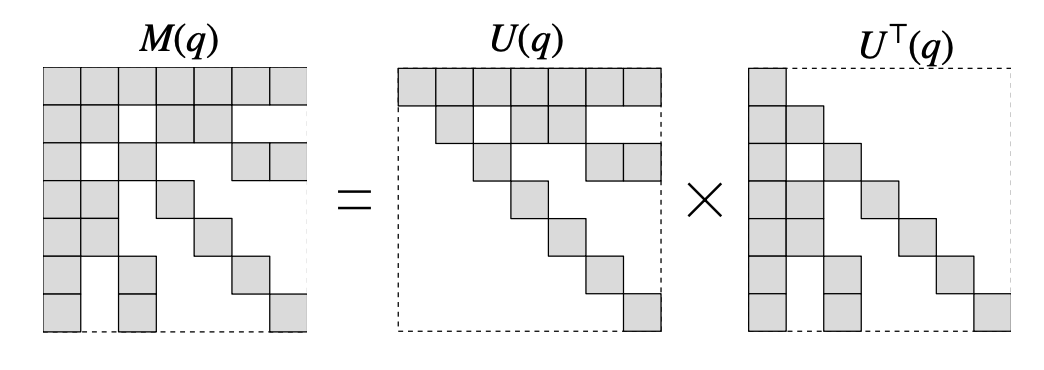
\includegraphics[width=.7\textwidth]{direct-inverse-dynamics/cholesky.png}
\end{figure}
This reduced the complexity to $O(n^2)$ when using a dense Cholesky decomposition.

\subsubsection{The maximum dissipation principle}
We showed that the contact forces $\lambda_c$ fulfill the relation:
\begin{equation*}
    G_c(q)\lambda_c + a_{c, f}(q, \dot{q}, \ddot{q}_f) = 0
\end{equation*}
From an energetic point of view, this solution minimizes:
\begin{equation*}
    \min_{\lambda_c} \frac{1}{2}\lambda_c^\tp G_c(q)\lambda_c + \lambda_c^\tp a_{c, f}(q, \dot{q}, \ddot{q}_f)
\end{equation*}
This is equivalent to the \emph{maximum dissipation principle}, which states that the contact forces are chosen to maximize the energy dissipation in the contact. This corresponds to the dual problem of the least-action principle, formally:
\begin{equation*}
    \max_{\lambda_c} -\frac{1}{2}\underbrace{
        \left(
            G_c(q)\lambda_c+2\lambda_C^\tp a_{c, f}(q, \dot{q}, \ddot{q}_f)
        \right)
    }_{a_c(q, \dot{q}, \ddot{q}_f)}
\end{equation*}
which is the dual of the least-action principle (primal):
\begin{equation*}
    \min_{\ddot{q}} \frac{1}{2}\norm{\ddot{q}-\ddot{q}_f}^2_{M(q)} \quad\text{s.t.}\quad J_c(q)\ddot{q} + \gamma_c(q, \dot{q}) = 0
\end{equation*}

\subsection{Rigid unilateral contacts}
\subsubsection{Unilateral contact as a Nonlinear Complementarity Problem}
The rigid unilateral contact model is used when the contact between the robot and the environment is rigid, and when the robot can only push the environment. This is the case, for instance, when the robot is standing on the floor. 

When dealing with unilateral contact conditions, three conditions must be satisfied:
\begin{enumerate}
    \item \textbf{Maximum dissipation} states that the contact forces should dissipate at most the kinetic energy:
    \begin{equation*}
        \min_{\lambda_c} \frac{1}{2}\lambda_c^\tp G_c(q)\lambda_c + \lambda_c^\tp a_{c, f}(q, \dot{q}, \ddot{q}_f)
    \end{equation*}
    \item \textbf{Complementary condition} (Signorini's conditions) require that the floor can \textbf{only push} (no pulling), and should emit no force when the contact is about to open:
    \begin{equation*}
        0\leq\lambda_{c,n} \perp a_{c,n}\geq 0
    \end{equation*}
    \item \textbf{Friction cone constraint} (Coulomb law) bounds the lateral forces by the normal force:
    \begin{equation*}
        \sqrt{\lambda_{c,x}^2 + \lambda_{c,y}^2} \leq \mu\lambda_{c,n}
    \end{equation*}
\end{enumerate}

\begin{figure}[H]
    \centering
    \begin{minipage}{0.4\textwidth}
        \centering
        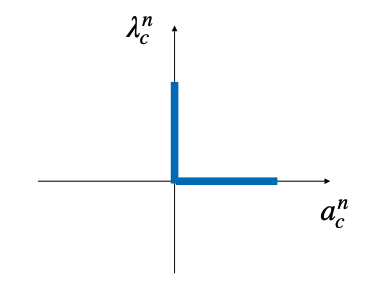
\includegraphics[width=.9\textwidth]{direct-inverse-dynamics/signorini.png}
        \caption*{Signorini's conditions}
    \end{minipage}
    \begin{minipage}{0.4\textwidth}
        \centering
        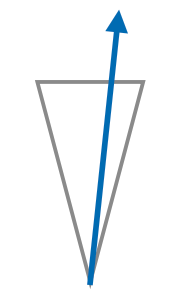
\includegraphics[width=.43\textwidth]{direct-inverse-dynamics/coulomb.png}
        \caption*{Coulomb law}
    \end{minipage}
\end{figure}

The contact problem then corresponds to a \emph{Nonlinear Complementarity Problem (NCP)}:
\begin{equation*}
    \begin{cases}
        \min_{\lambda_c} \frac{1}{2}\lambda_c^\tp G_c(q)\lambda_c + \lambda_c^\tp a_{c, f}(q, \dot{q}, \ddot{q}_f) \\
        0\leq\lambda_{c,n} \perp a_{c,n}\geq 0 \\
        \sqrt{\lambda_{c,x}^2 + \lambda_{c,y}^2} \leq \mu\lambda_{c,n}
    \end{cases}
\end{equation*}
which is non-convex, hence hard to solve. More complex solvers can be used to solve this problem in an exact way.

\subsubsection{Relaxed contact problem}
Another approach to solve the rigid unilateral contact problem is to relax the contact conditions. This is done by removing the complementarity condition, and by regularizing the forces:
\begin{equation*}
    \begin{cases}
        \min_{\lambda_c} \frac{1}{2}\lambda_c^\tp (G_c(q)\textcolor{red}{+R})\lambda_c + \lambda_c^\tp a_{c, f}(q, \dot{q}, \ddot{q}_f) \\
        \sqrt{\lambda_{c,x}^2 + \lambda_{c,y}^2} \leq \mu\lambda_{c,n}\\
        \hcancel[red]{0\leq\lambda_{c,n} \perp a_{c,n}\geq 0}
    \end{cases}
\end{equation*}
where $R$ is a regularization term. This problem becomes convex, which makes it much easier to solve. Nevertheless, the solution is not exact, which might lead to some physical inconsistencies.

\subsection{Inverse dynamics}
Similarly to the inverse kinematics problem, we can solve the inverse dynamics problem by minimizing the gap between the actual motion of the robot and the desired motion. Instead of solving for the configuration of the robot, $q\in Q$, we solve for the forces applied to the robot, or equivalently for $\ddot{q}, \tau, \lambda_c$.

Consider the actual position and speed of the end effector, $(M, v, a)$. To compare it to a reference trajectory $(M^*, v^*, a^*)$, we define the error as:
\begin{equation}
    e := M\ominus M^* = \log_{\SE(3)}\left((M^*)^{-1}M\right)
\end{equation}
The error in velocity space is given by:
\begin{equation*}
    \dot{e} = v - v^*
\end{equation*}
and the acceleration of the error is:
\begin{equation*}
    \ddot{e} = a - a^* = J(q)\ddot{q} + \dot{J}(q, \dot{q})\dot{q} - a^*
\end{equation*}
This allows us to define the error correction profile as:
\begin{equation}
    \ddot{e}=-K_pe-K_v\dot{e}
\end{equation}
for some $K_p, K_v>0$. We can then solve the following optimization problem:
\begin{equation*}
    \min_{\ddot{q},\tau,\lambda_c} \frac{1}{2}\norm{\ddot{e}+K_p\dot{e}+K_v\dot{e}}_2^2 \quad\text{s.t.}\quad M(q)\ddot{q} + C(q, \dot{q}) + G(q) = \tau + J_c^\tp(q)\lambda_c
\end{equation*}
with $\lambda_c$ the contact forces.
\section{Motion planning}
\subsection{Configuration space}

\section{Collision Detection}
Collision detection is a subject at the center of physics simulators. To build a simulation of the robot in its environment, the main loop goes as follows:
\begin{enumerate}
    \item Collision detection: finding contact points
    \item Collision resolution: finding contact forces using physical principles
    \item Time integration: update of the quantities of interest (position, velocity, etc.)
\end{enumerate}
It is therefore crucial to have an efficient collision detection algorithm, that is to know whether two objects are in contact or not, and if so, to find the contact points.

Nevertheless, collision detection is a computational bottleneck in physics simulators. Resolving collision detection for one pair of objects takes a significant amount of time, especially for complex shapes, and the number of pairs to check grows quadratically with the number of objects. A general method to optimize such a process is to decompose one collision detection into two phases, the broad phase and the narrow phase. The broad phase uses simple geometric primitives to quickly discard pairs of objects that are far from colliding. The narrow phase then uses more complex geometric primitives to find the exact contact points.

\subsection{The broad phase}

\subsection{The narrow phase}

\newpage
\section{Optimal Control}
% \section{Reinforcement Learning}
% \section{Locomotion}

\end{document}